\documentclass[11pt,letterpaper]{article}

\usepackage{tabularx,booktabs}
\usepackage{url}
\usepackage{fullpage}
\usepackage{graphicx}
\usepackage{lipsum}
\usepackage{amsmath}
\usepackage{algorithm,algpseudocode}
\newcommand{\junk}[1]{}

\begin{document}
\thispagestyle{empty}

\title{RECOMB paper template}
\author
{
\centering
Master$^{1}$ \and Yoda$^{2}$ \and Doctor$^{1}$\footnote{Corresponding Author. Email: thirteenth@doctorwho.com} 
\\
		$^{1}$Dept of Dalek Affairs, Time Lord Academy, 42424 Gallifrey\\
	   	$^{2}$Dept of Light Saber Engineering, Jedi Academy, 12345, Coruscant\\	
}

\date{}

\maketitle
\begin{abstract}
Identifying the genome functions is one of the main challenges in the field of biology. However it has been more than a decade that the sequencing of the human genome has clarified a significant portion of genome functions but much is still unknown.\\
One of the most effective ways for understanding the mechanism of the transcriptional regulation is through identifying the transcription factor binding sites. Various experimental and computational approaches have been used to detect these sites. Here we are going to introduce a novel method for identifying these sites.
\end{abstract}

\section{Introduction}
A primary function of the genome is the production of RNA transcripts of
genes, which go on to produce the proteins that carry out most cellular activity\cite{muto2002transcription}. Gene regulation
occurs through a number of biochemical processes. In the cell, most DNA is wrapped around 
histone proteins, forming a DNA-protein complex called chromatin. DNA-binding proteins (transcription
factors) act on chromatin, changing its biochemical activity by recruiting other factors,
covalently altering histone proteins, moving and removing histones to reveal the underlying DNA,
and ultimately expressing or silencing a given gene. This complicated process is a key determinant
of human traits, evolution and disease\cite{chi2010covalent}.\\
In order to capture the gene regulation, experimental methods know as genomic assays have emerged.
These experimental assays leverage DNA sequencing technology to assay various
types of biochemical properties.\\
Some of the known genomic assays which have accelerated the process of identifying gene regulation are transcription factor chromatin immunoprecipitation sequencing (TF CHIP-seq) which aims to identify the binding sites of a given transcription factor and histone CHIP-seq as another kind of sequencing which aims to identify gene requlation.\\
In a ChIP-seq experiment, the researcher applies a series
of biochemical reactions to break up the genome into small fragments of DNA, then applies an
antibody to extract the fragments that are bound to a certain transcription factor (the term “immunoprecipitation” derives
from this antibody step). The researcher then uses DNA sequencing technology to read the DNA
sequence of each fragment. This sequence is known as a “read”. If that sequence occurs exactly
once in the human reference genome, the read is taken as evidence that the transcription factor
binds to the matching position\cite{overballe2012next}.\\
One of the most important functional elements in any
genome is transcription factor binding sites, the sites within
the DNA to which they bind. These interactions between
protein and DNA control many important processes, such as
critical steps in development and responses to environmental
stresses, and defects in them can contribute to the progression
of various diseases\cite{baxevanis2004bioinformatics}.\\
Therefore, identifying these sites is one of the enormous challenges.
Many computational approaches have been proposed for addressing this issue which in the following, some of the most important ones are introduced briefly.\\
Kharchenko et al. developed a ChIP-seq processing pipeline (spp) which was designed to detect protein-binding positions with high accuracy by introducing methods to improve tag alignment\cite{kim2011short}.
Spp implemented three peak-calling methods: (1) the
window tag density (WTD) is a method that extends positive- and
negative-strand tags by the expected DNA fragment
length in order to determine binding positions to
those tags with the highest number of overlapping
fragments, and scores positions based on the strandspecific
tags; (2) the matching strand peaks (MSP)
approach (which determines local peaks of strandspecific
tag density and identifies positions surrounded
by positive- and negative-strand peaks); (3)
the mirror tag correlation (MTC) method (which
scans the genome to identify positions exhibiting
pronounced positive- and negative-strand tag patterns
that mirror each other). All methods employ background
subtraction of the control tag density to
correct for the uneven background distribution. The
p-value is calculated assuming Poisson density, and
candidate binding sites were selected with p-values < $10^{-5}$.
Given the score s calculated by one of the
above methods, the corresponding false discovery rate
(FDR) can be estimated as the number of binding
positions with the score s or higher found in the
ChIP dataset, divided by that in the control set\cite{kharchenko2008design}.\\
Jiang et al. developed a tool, CisGenome, for ChIP data analysis. This approach uses a conditional binomial model for two-sample analysis\cite{ji2008integrated}.
Another approach which is one of the most well-known approaches in identifying transcription factor binding sites is Model-based Analysis of ChIP-Seq (MACS)\cite{zhang2008model}.
The idea behind MACS approach is to move all peak by $d/2$ toward the 3' end in which $d$ is the distance between two peaks of the positive and negative strands.
In the following, we are going to describe our proposed method and we are going to compare our method to two other well-known approaches.  
\section{General strategy for identifying transcription factor binding sites}
ChIP-seq Experiments for identifying transcription factor binding sites can generally fall into two categories: One-sample and two-sample experiments\cite{kim2011short}.
Only one ChIP sample is sequenced in the one-sample analysis but despite the one-sample analysis, a control sample is sequenced in two-sample studies in addition to the ChIP sample and this is due to the some biases from random protein-DNA or antibody-DNA interactions,etc.
Therefore, because of these biases, two-sample analysis is needed for a more reliable results.
Here in this project, We have used two replicates for our analysis.
In the following, the general strategy for identifying the peaks from ChIP-seq data are described.
\subsection{Creating the signal profile}
As it was mentioned before, we have used two replicates in order to produce the natural unit for getting the signal profiles for each of the tags in the replicates.
Each of the tags in the replicates show specific position in the genome with their corresponding signal which describes the tag's significance to be the precise position of the transcription factors.
Many computational and experimental methods have proposed different approaches for getting these signals and here in this project, we have used the variance-stabilization method in order to get these signals.
%\subsubsection{Variance-Stabilization Method}                   
In order to understand genome activity, it is important to be able to ask whether or not a given drug, tissue, or disease produces a statistically significant change in activity relative to a particular cellular condition. This question is difficult to answer because the output of a genomics assay---the number of reads mapping to a given genomic position---has no natural units. In particular, a difference between 0 and 30 reads may have a very different statistical importance from a difference between 1,000 and 1,030 reads. This property is due to a relationship between the mean of the data-generating process (i.e. the genomics assay) and its variance.\\ Currently-used models that do not model this mean-variance relationship, such as a Poisson model, result in poor evaluation of statistical differences. We plan to develop a method to learn the mean-variance relationship of functional genomics data sets using the variation among biological replicates.\\
Learning the mean-variance relationship of these data sets has the benefit that it makes it possible to place genomics data in interpretable units. The lack of natural units for genomics data sets makes it difficult to analyze these data sets by eye and confounds any downstream analysis that does not internally model the mean-variance relationship (such as genome annotation). Currently, as a preprocessing step, many analyses of genomics data sets transform the data using a log or inverse hyperbolic sine transform to attempt to normalize for the mean-variance relationship of the sequencing read counts. However, there is no theoretical basis for using these particular transformations rather than any other, so they almost certainly do not properly account for the mean-variance relationship as intended. Given a known mean-variance relationship, a data set can be put into interpretable units using the variance-stabilizing transformation $f(x) = \int \frac 1 {\sigma(u)} du$, where $\sigma(x)$ is the standard deviation of a variable with a mean of $x$. The resulting signal is in units of standard deviation, so it has the useful property that all data points have a 95\% confidence intervals of $\sim$2 units. Therefore, variance-stabilized data sets are a natural by-product of a principled method for evaluating statistical differences. These data sets are much more easily analyzed by eye, and are necessary for any downstream analysis that does not internally model the mean-variance relationship.
The distribution of the signals among tags between two replicates is shown in the figure \ref{fig:go1}.
%\begin{figure}[h]
%	\begin{center}
%		\includegraphics[scale=.3]{CTCFplot.pdf}
%		\vspace*{8pt}
%		\caption{Tag signals in two replicates}
%		\label{fig:go1}
%		
%	\end{center}
%\end{figure} 
In the next step, we are going to find the mean-variance relationship between the two replicates.
For this purpose, we need to consider enough segments of the data between two replicates. In this project, we have decided to consider 1000 points in each step from each of the replicates to build the mean-variance relation between two replicates.
For selecting the specific number of points to be considered as a part of mean-variance relation curve, we need to use a slide window with the width of 1000 to scan the genomic positions across the genome. We begin the procedure by selecting 1000 points from the lowest signals in replicate 1 and their corresponding signal for the specific position from the replicate 2.
By computing the mean and variance of these data, we get the mean-variance relation as it is shown in the figure \ref{fig:go2}.
%\begin{figure}[h]
%	\begin{center}
%		\includegraphics[scale=.6]{mean-var.PNG}
%		\vspace*{8pt}
%		\caption{Relation between mean-variance between two replicates}
%		\label{fig:go2}
%		
%	\end{center}
%\end{figure}
After identifying the mean-variance relation, we need to introduce new signals for each tag in the replicates.
For this purpose, we have used the variance-stabilization method for computing the new signals.
Therefore, introduced signals for each tag is computed as the area under the mean-variance curve in the [0,signal] interval, which signal is the tag's score in each replicates. New signals are computed as the following equation.\\
\begin{equation}
f(x) = \int_{0}^{x}\text{mean-variance curve}
\end{equation}
which in this equation, $x$ shows the tags raw signal from each of the replicates.
\subsection{Selecting the peaks}
After creating the signal profile for each of the replicates, we are going to introduce the top ranked signals as the candidate binding sites.
\subsection{Evaluating the significance of peaks}
In this part, we need to calculate the significance of the identified peaks and to see whether these peaks are reliable enough to introduce them as transcription factors.
Therefore, we are going to see whether the candidate binding sites match the known motifs for the specific transcription factors or not. 
In the following, psudo code for our proposed method has been provided.
\begin{algorithm}[h]
	\caption{Mean-Variance stabilization approach}
	\begin{algorithmic}[1]\baselineskip=14pt\relax
		\State  \textbf{Input:} Two replicates from fold enrichment analysis, Number of points in each segment $(n)$, Number of the candidate binding sites $(N)$.
		\State  \textbf{Output:} List of candidate transcription factor binding sites.
		\State Sort the signals in replicate 1
		\For{$i=1, 2,..., (length((replicate 1)/n))$}
		\State Select $n$ points from replicate 1 and their corresponding point in the genome position.
		\State Calculate the mean and variance for $n$ $(replicate 1, replicate 2)$ points
		\EndFor
		\For{$i=1,2,...,(length(replicate 1))$}
		\State Calculate new signal for each of the replicate 1's tags from fold enrichment analysis by computing the area under the curve of the mean-variance curve in the $(0,replicate 1 signal(i))$ interval.
		\EndFor
		\For{$i=1,2,...,(length(replicate 2))$}
		\State Calculate new signal for each of the replicate 2's tags from fold enrichment analysis by computing the area under the curve of the mean-variance curve in the $(0,replicate 2 signal(i))$ interval.
		\EndFor
		\State Return $N$ highest ranked signals for each of the replicates as the candidate binding sites.
	\end{algorithmic}
	\label{alg:mean-var}
\end{algorithm}
\section{Materials}
\subsection{Dataset}
Here in this project, we are going to use the ChIP-Seq data for two transcription factors: NRSF factor and CTCF factor.
Two replicates for NRSF transcription factor are obtained from REST ChIP-seq protocol PCR2x on human GM12878 and replicates for CTCF are from CTCF ChIP-seq on human GM12878
\subsection{Method comparison}
We compared our method with two other methods; ChIP processing pipeline(spp) and data derived from the fold enrichment analysis.
Due to the huge amount of the identified tags for transcription factors, we compared our results just for Chromosome 21 in each method.\\
We compare our results by determine the accuracy of the proposed methods in identifying the transcription factor binding sites. For this purpose, we are going to calculate the motif occurrence for each of the TF factors.
\section{Results and discussion}
As it was mentioned before, we have used two transcription factors in our analysis.
The two replicates of the CTCF have 395440 and 276976 read tags respectively and two replicates of NRSF have 619610 and 518673 read tags.
CTCF factor has 9657 known motifs and NRSF factor has 460 know motifs.
We have compared our proposed method to two other methods: SPP and fold enrichment analysis.
Since SPP method have introduced 3000 and 2000 candidate binding sites for each of the replicates in CTCF and NRSF factors, therefore we decided to introduce the same number of the candidate peaks for each factor. As it was mentioned before, the highest ranked signals are considered as the candidate peaks
\subsection{Motif occurance analysis}

%For determining the accuracy percentage of each method, we have measured the percentage of predicted peaks with the known motifs within 50 base pair(bp) of the peak summit of the motifs.
\begin{table}[h] 
	\caption{Number of the true predicted binding sites of each method for CTCF factor}
	\centering 
	\scalebox{0.99}{
		\begin{tabular}{|l| c| c | }
			\hline 
			
			Methods & Replicate 1 & Replicate 2
			\\\hline
			
			SPP	&	953/3000&	713/2000	
			\cr{Fold enrichment}	&	2520/3000&	1499/2000
			\cr{Mean-variance stabilization}	&2520/3000	&	1510/2000 \\
			\hline
		\end{tabular}
	}
	\label{tab:CTCF}
\end{table} 
%=====================================================================

%===========================================================================
%The results that we got from all three methods were not good enough and even SPP which is one of the well-known methods in identifying transcription factor binding sites had poor prediction.
%The reason was totally not clear.
%Therefore we decided to compare the frequency of the known motifs from each replicate with the frequency of the signals in whole genome.
%For this purpose, we used the NRSF factor replicates to identify their motifs. So we implemented a brute force procedure for each of the two replicates and compared them with the known motifs for NRSF factor in order to get the real motifs of these replicates.
%Finally, we identified 1244 binding sites from replicate 1 and 1110 binding sites from replicate 2 that match with the known motifs for NRSF factor. 
%The histogram for NRSF replicates signal frequency are shown in figures \ref{fig:go3} and \ref{fig:go5} and the histogram for the NRSF motif frequency in two replicates are shown in the figures \ref{fig:go4} and \ref{fig:go6}.
%By comparing these histograms, we realized that the hypothesis about selecting the highest ranked signals as the candidate binding site may not be true and in our experiment, points with signals smaller than the mean of the signals have been identified to be the true transcription factor binding sites.
%Therefore, we believe that our proposed method might not be good enough in this stage to be considered as a transcription factor binding site predictor and we will strongly try to consider new insights in our proposed method in order to increase its performance and make it a reliable approach.   
%=====================================================================
\subsection{Gene expression analysis}
\begin{table}[h] 
	\caption{Spearman Correlation Coefficient}
	\centering 
	\scalebox{0.99}{
		\begin{tabular}{|l| c| c | }
			\hline 
			
			Methods & CTCF GM12878 &  H3K4me3 GM12878
			\\\hline
			
			%SPP	&	19/460&	16/460	
			Fold enrichment	&	0.05972792&	0.3231677	
			\cr{Mean-variance stabilization}	&	-0.006524079&	0.3210593 \\	
			\hline
		\end{tabular}
	}
	\label{tab:NRSF}
\end{table} 






\begin{table}[h] 
	\caption{Pearson Correlation Coefficient}
	\centering 
	\scalebox{0.99}{
		\begin{tabular}{|l| c| c | }
			\hline 
			
			Methods & CTCF GM12878 &  H3K4me3 GM12878
			\\\hline
			
			%SPP	&	19/460&	16/460	
			Fold enrichment	&	0.05043497&	0.4562976	
			\cr{Mean-variance stabilization}	&	0.03759687&	0.4230482\\	
			\hline
		\end{tabular}
	}
	\label{tab:NRSF}
\end{table} 

%=============================
\subsection{Differentially expression analysis}
\begin{table}[H] 
	\caption{ROC-AUC}
	\centering 
	\scalebox{0.99}{
		\begin{tabular}{|l| c| c | }
			\hline 
			
			Methods & CTCF GM12878-K562 &  H3K4me3 GM12878-K562
			\\\hline
			
			%SPP	&	19/460&	16/460	
			Fold enrichment	&	0.5667&	0.6752	
			\cr{Mean-variance stabilization}	&	0.498&	0.6938\\	
			\hline
		\end{tabular}
	}
	\label{tab:NRSF}
\end{table} 

%============================
\begin{figure}[H]
	\begin{center}
		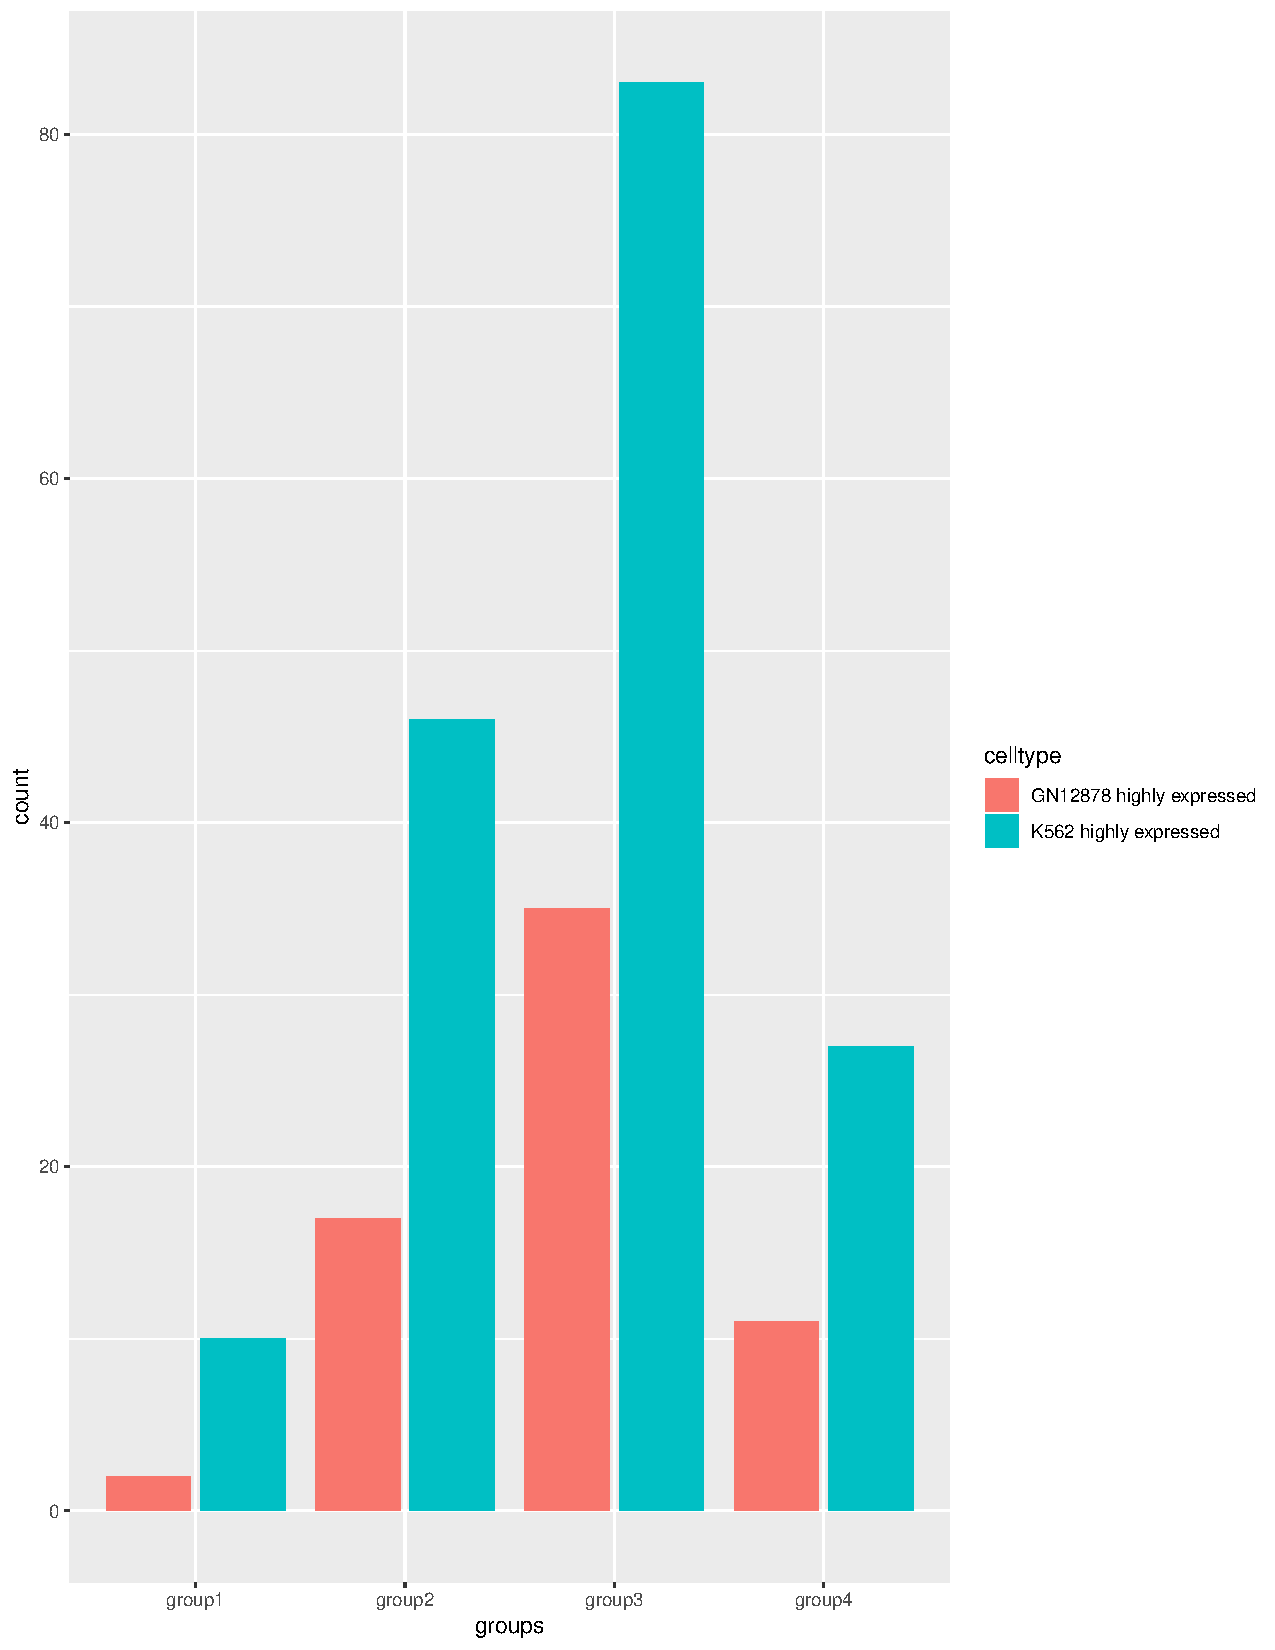
\includegraphics[scale=.3]{FE-CTCF-GM12878-K562.PDF}
		\vspace*{8pt}
		\caption{GM12878 and K562 quantitative differences in CTCF in fold enrichment method}
		\label{fig:go2}
		
	\end{center}
\end{figure}


\begin{figure}[H]
	\begin{center}
		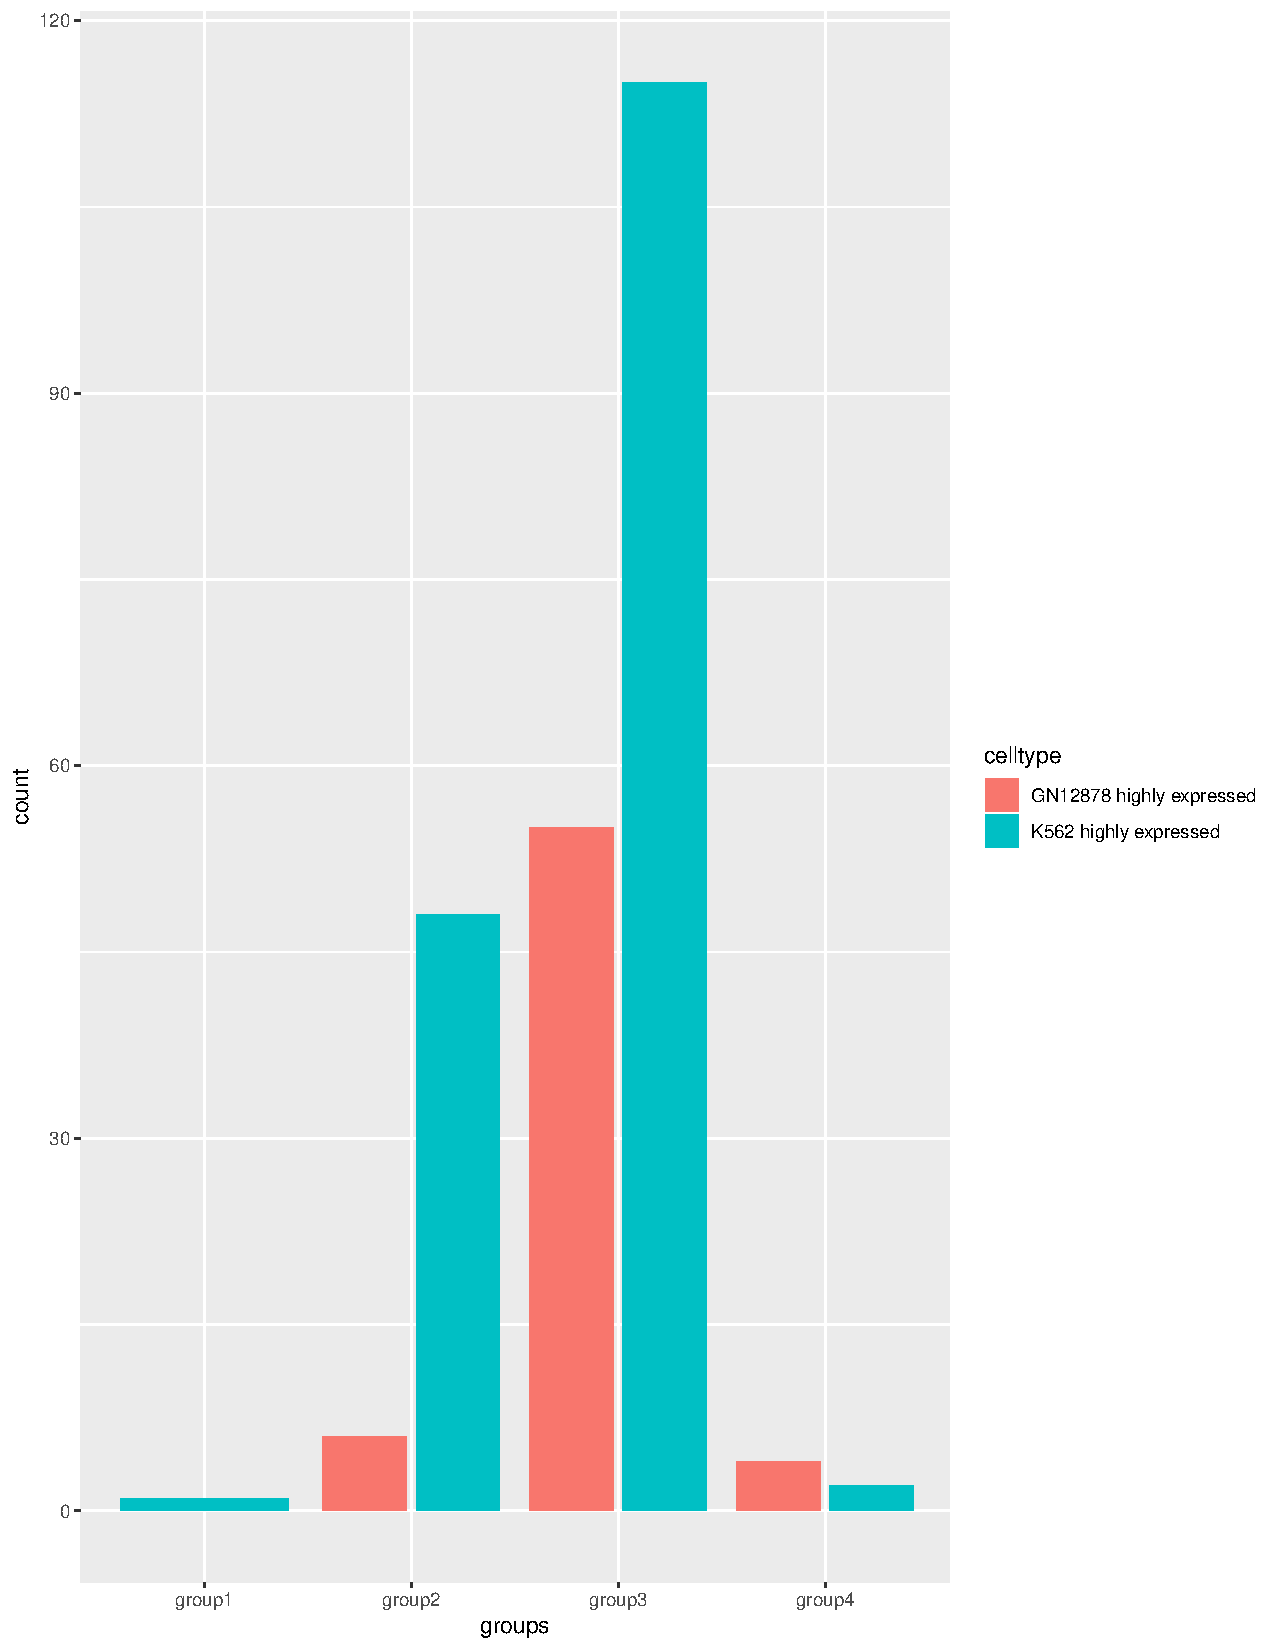
\includegraphics[scale=.3]{FE-H3K4me3-GM12878-K562.PDF}
		\vspace*{8pt}
		\caption{GM12878 and K562 quantitative differences in H3K4me3 in fold enrichment method}
		\label{fig:go2}
		
	\end{center}
\end{figure}


\begin{figure}[H]
	\begin{center}
		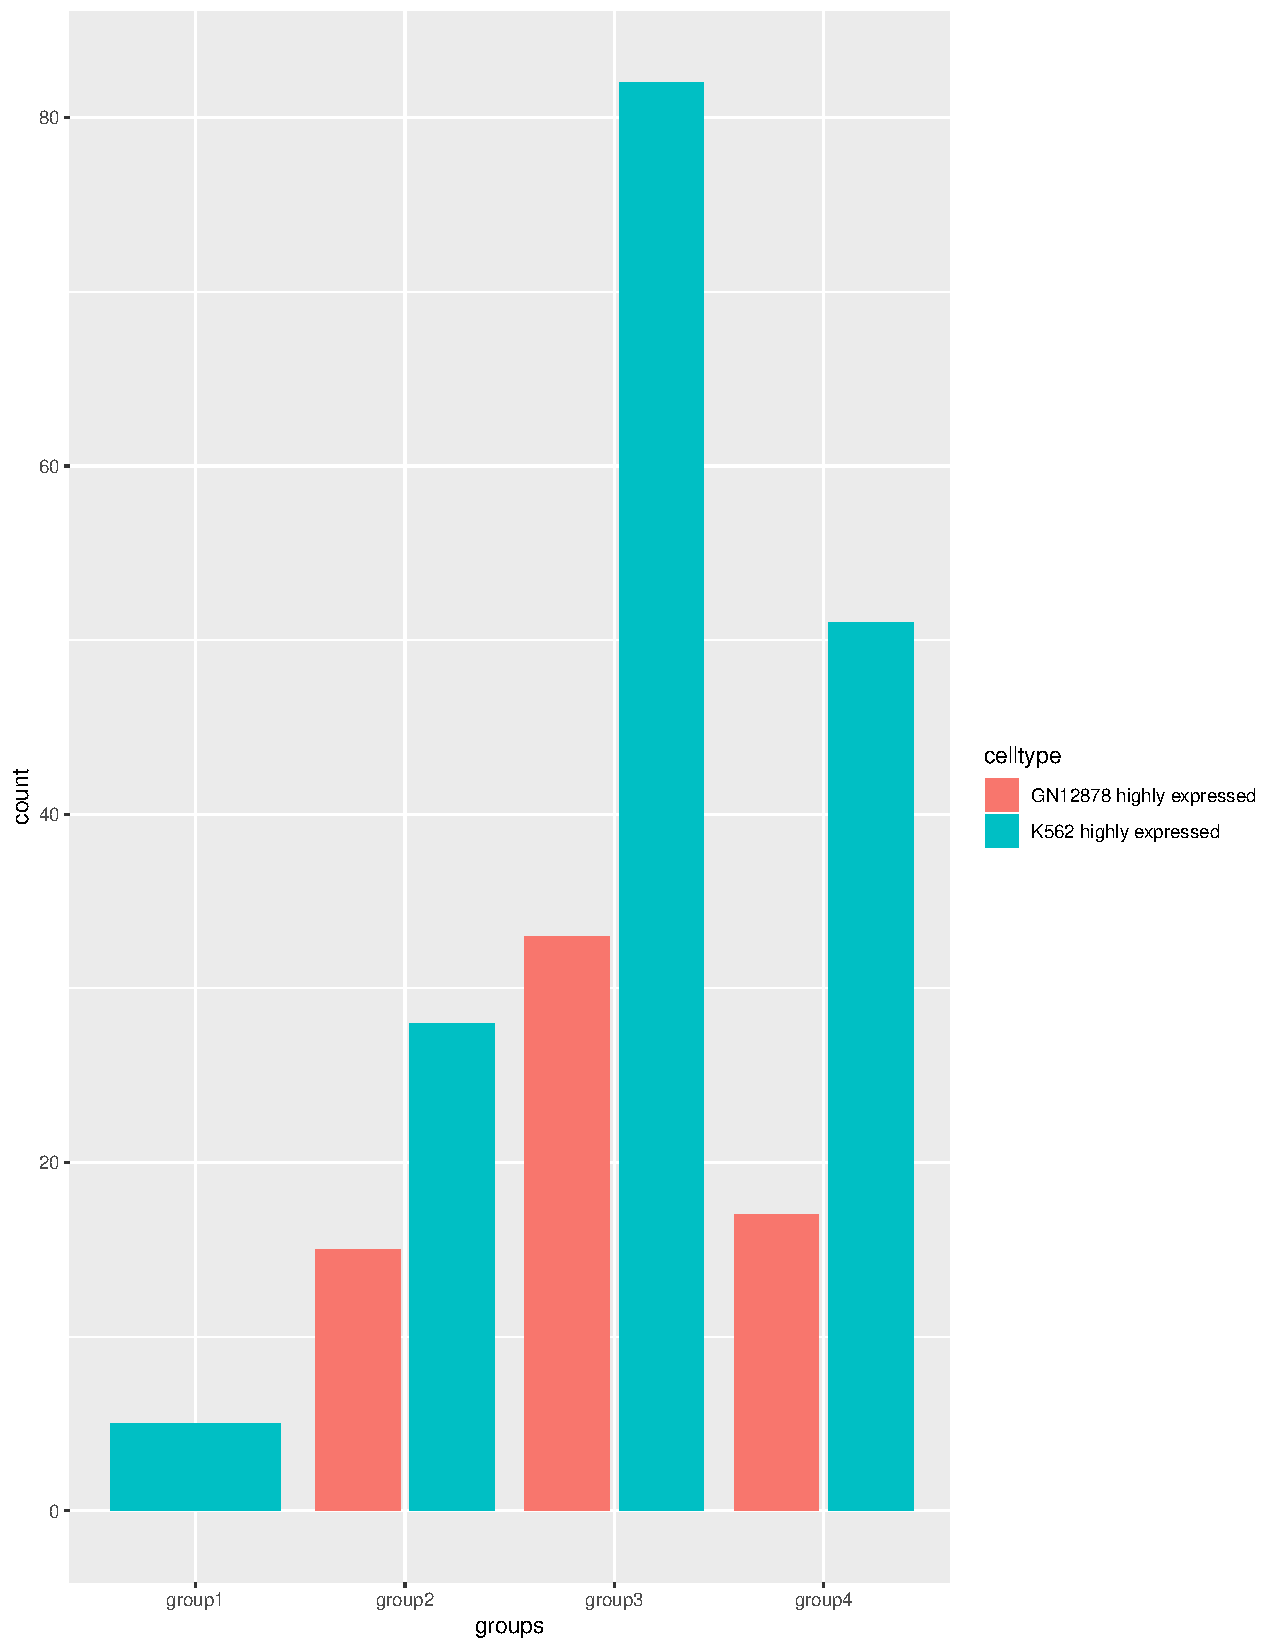
\includegraphics[scale=.3]{MV-CTCF-GM12878-K562.PDF}
		\vspace*{8pt}
		\caption{GM12878 and K562 quantitative differences in CTCF in mean-variance stabilization method}
		\label{fig:go2}
		
	\end{center}
\end{figure}


\begin{figure}[h]
	\begin{center}
		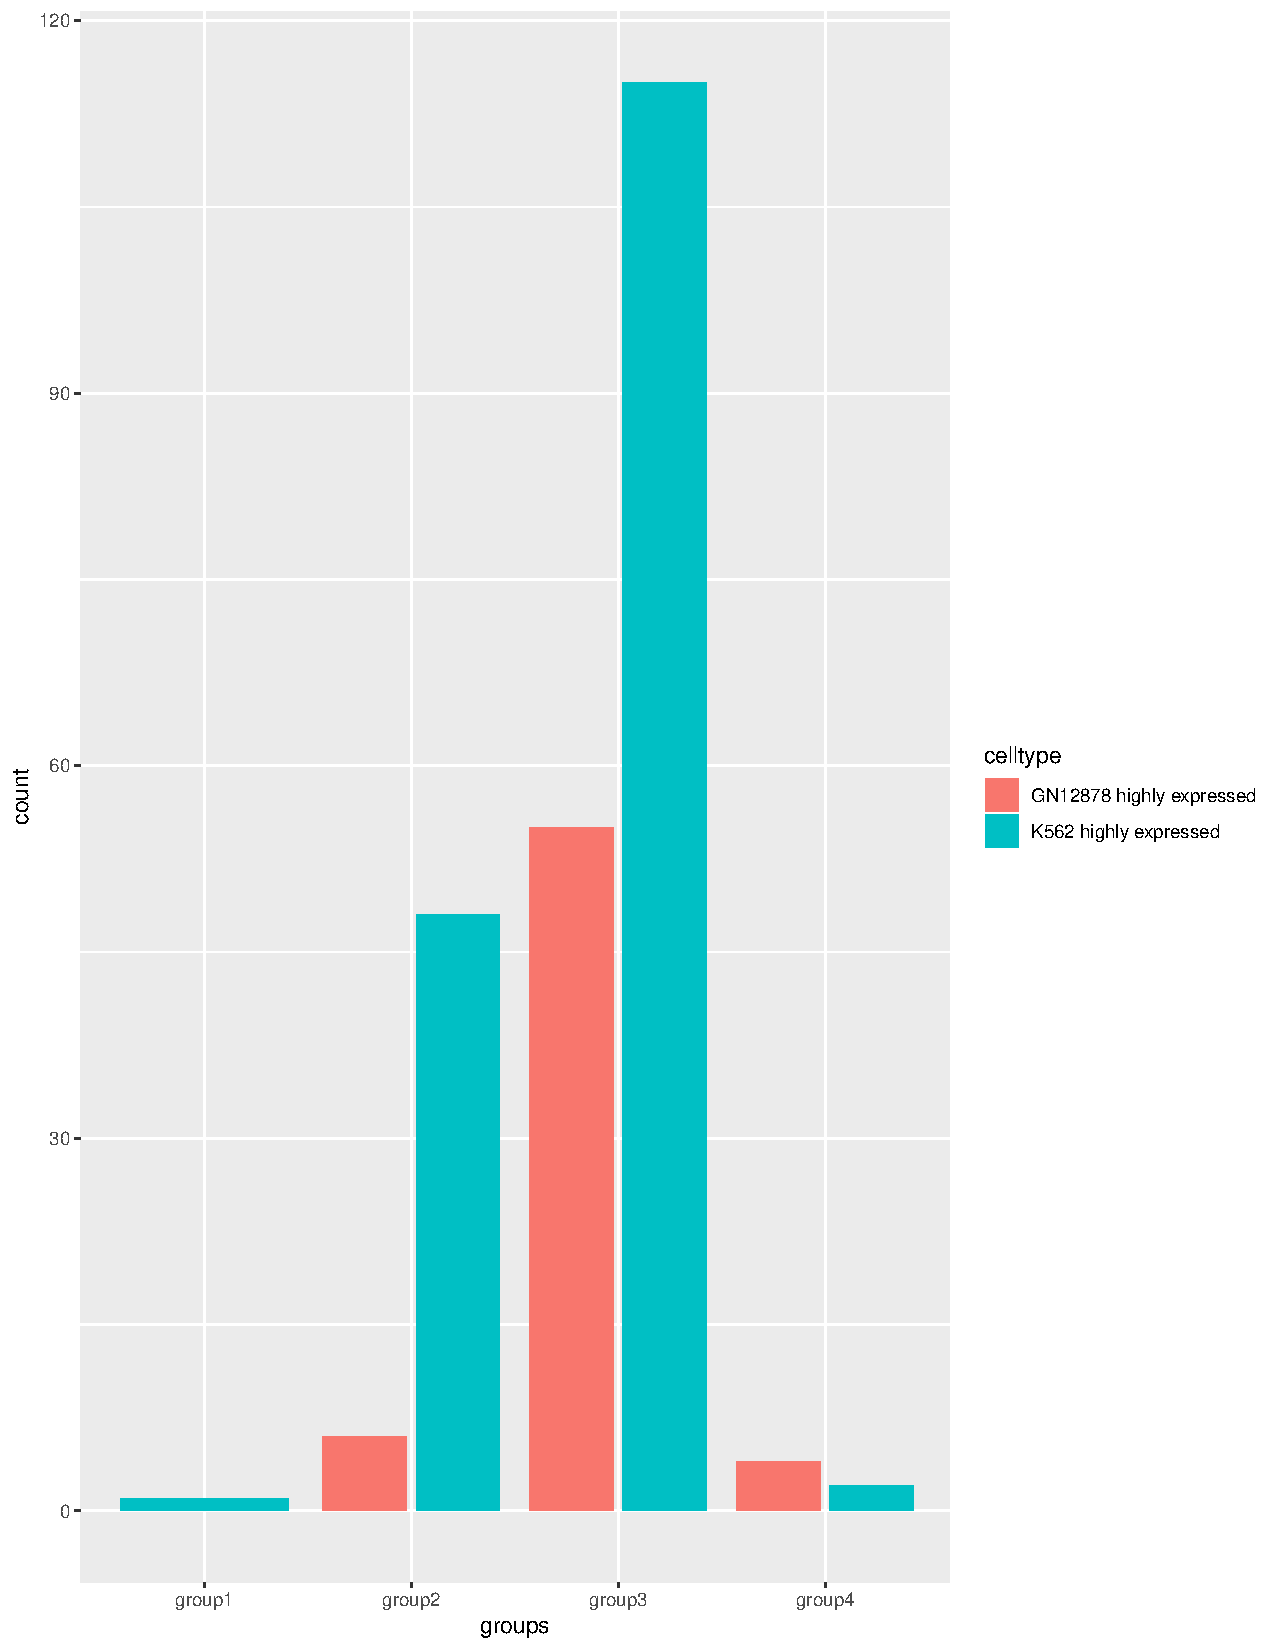
\includegraphics[scale=.3]{FE-H3K4me3-GM12878-K562.PDF}
		\vspace*{8pt}
		\caption{GM12878 and K562 quantitative differences in H3K4me3 in mean-variance stabilization method}
		\label{fig:go2}
		
	\end{center}
\end{figure}


\section{Conclusion}
In this project, we tried to introduce a new approach for predicting precise locations for transcription factor binding sites.
The idea behind our method is that we would like to propose a new scoring method so that all data sets have natural units and therefore interpreting these data might be much more easier even by eye.
Therefore, we proposed a new method called mean-variance stabilization method and we believed that the results of the proposed method may be better than the other approaches but during our project we realized that not even our method but also other well-known approaches are facing a problem in the peak calling procedure. Because all the methods consider the highest ranked signals as the true binding sites but our experiments showed that it may not guarantee that by selecting the highest ranked signals we have achieved true results.
So, in this stage, we believe that we need to take into account more properties for identifying the transcription factor binding sites.  
\section{Future Work}
%As it was mentioned in the results section, it seems that selecting the highest ranked signals in the read tags doesn't guarantee that the candidate binding sites are true binding sites for the transcription factors and results show this interpretation which was so strange because even SPP as one of the most well known methods in identifying transcription factor binding sites, show poor identification and results.
%Therefore, we believe that we should take in mind this property and design more reliable methods that consider low signals of the tags in the process of identifying transcription factors. 


\section{Acknowledgements} 
This work was supported by a grant by ...

\bibliographystyle{myrecomb}

\bibliography{mybib}

\end{document}


